\documentclass[a4paper, 12pt]{extarticle}

\usepackage{packages}
\usepackage{environments}
% \usepackage{commands}
% \usepackage{appearence}
\renewcommand{\baselinestretch}{1.5}
\addbibresource{library.bib}
\setlength{\parindent}{1.25em}

\usepackage{tocloft}

\begin{document}

    \begin{titlepage}
\thispagestyle{empty}
\setlength{\parindent}{0ex} % set paragraph indenting to zero

\newgeometry{top=18.3mm,left=30mm,right=14.8mm,bottom=0.49mm}

\headsep=3.8pt

\begin{center}
  {\small {\bf ПРАВИТЕЛЬСТВО РОССИЙСКОЙ ФЕДЕРАЦИИ \\
  ФГАОУ ВО НАЦИОНАЛЬНЫЙ ИССЛЕДОВАТЕЛЬСКИЙ УНИВЕРСИТЕТ \\
  <<ВЫСШАЯ ШКОЛА ЭКОНОМИКИ>>}\\[13.75pt]
  Факультет компьютерных наук \\
  Образовательная программа <<Прикладная математика и информатика>>}
\end{center}

\vspace{-1.8ex}

{\small УДК \line(1, 0){3cm} }

\vspace{75pt}

\begin{center}
  {{\fontsize{12}{\baselineskip}\selectfont \bf Отчет об исследовательском проекте \\[5.95pt]}
  на тему <<Топологический анализ социальных данных>> \\[10pt]
  (промежуточный, этап 2)}
\end{center}

\vspace{70.45pt}

{\bf Выполнил:}

\vspace{-2.8ex}

\begin{center}
    \hspace{0.5cm} {студент группы БПМИ 198} \hfill 
    $\overset{\displaystyle\text{\textcolor{white}{C.В. Пилипенко}}}{\underset{\text{\scriptsize Подпись}}
    {\line(1, 0){0.2\textwidth}}} \hspace{1em}
    \overset{\displaystyle\text{С.В. Пилипенко}}{\underset{\text{\scriptsize И.О. Фамилия}}
    {\line(1, 0){0.3\textwidth}}}$
\end{center}

\vspace{-2.3ex}

$\underset{\text{\scriptsize Дата}}{\underline{29.04.2021}}$

\vspace{44.5pt}

{\bf Принял:}

\vspace{-2.8ex}

\begin{center}
    \hspace{0.5cm} {руководитель проекта} \hfill 
    $\overset{\displaystyle\text{Айзенберг Антон Андреевич}}{\underset{\text{\scriptsize Имя, Отчество, Фамилия}}
    {\line(1, 0){0.66\textwidth}}}$ \\
    \hfill $\overset{\displaystyle\text{кандидат физико-математических наук, доцент}}{\underset{\text{\scriptsize Должность, ученое звание}}{\line(1, 0){0.963\textwidth}}}$ \\
    \hfill $\overset{\displaystyle\text{международная лаборатория алгебраической топологии и ее приложений}}{\underset{\text{\scriptsize Место работы (Компания или подразделение НИУ ВШЭ)}}
    {\line(1, 0){0.963\textwidth}}}$ \\[10 pt]
    Дата проверки $\overset{\displaystyle}{\underset{\text{\scriptsize }}{\line(1, 0){2cm}}} 2021 \hspace{1em} 
    \overset{\displaystyle}{\underset{\substack{\text{Оценка} \\ \text{(по 10-тибалльной шкале)}}}
    {\line(1, 0){0.25\textwidth}}} \hfill 
    \overset{\displaystyle}{\underset{\text{\scriptsize Подпись}}{\line(1, 0){0.25\textwidth}}}$ \\
\end{center}

\vspace{20pt}
\begin{center}
  {\bf Москва 2021 г.}
\end{center}

\restoregeometry

\setlength{\parindent}{1.25cm} % reset paragraph indenting
\end{titlepage}
    
    \setcounter{page}{2}
    \tableofcontents
    
    % \section{Реферат}

Наша работа была мотивированна изучением молодой и активно развивающейся областью топологии -- топологического анализа данных (TDA), возникшая посредством множества работ в вычислительной геометрии и прикладной топологии. 
В основе TDA лежит идея о том, что топология и геометрия обеспечивают крайне эффективный подход к получению надежной качественной и, иногда, количественной информации о структуре данных.
TDA стремится предоставить достаточно обоснованные математические, статистические и алгоритмические методы для вывода, анализа и использования топологических структур, лежащих в основе данных, которые часто представлены в виде точек в метрическом пространстве. 
Целью исследования нашей работы были социальные опросы школьников, руководителей и учителей с помощью которых мы надеялись выявить паттерны посредством использования методов TDA, в частности, UMAP и PCA.
В первом этапе работы, мы занялись очисткой данных от статистических выбросов и изучением методички по топологии, во втором этапе мы сформулировали гипотезы, изучили алгоритмы UMAP и PCA и реализовали их на наших, уже очищенных датасетах, в третьем этапе мы занялись обоснованием корректности нашей работы.
Результаты нашей работы показали, что ответы участников опроса не зависели от пола, класс учеников не влиял на их мнение и распределение ответов сотрудников школьной администрации не зависит от должности.
            % Реферат (краткий обзор исследования, -- зачем, почему, как и что вышло)
    \section{Основые термины и определения}

\begin{description}
    \item[Метрическое пространство] {\it Метрическим пространством} $(M, \rho)$ называют множество $M$ с функцией $\rho: M \cross M \rightarrow \mathbb{R}_{+}$, называющейся расстояние, для любых $x, y, z \in M$, что:
    \begin{enumerate}
        \item $\rho(x, y) \geq 0$ и $\rho(x, y) = 0$ iff $x = y$
        \item $\rho(x, y) = \rho(y, x)$
        \item $\rho(x, z) \leq \rho(x, y) + \rho(y, z)$
    \end{enumerate}
    \item[Симплициальный комплекс] {\it Симплициальным комплексом} на конечном множестве вершин $M$ называется совокупность $K \subset 2^{M}$ подмножеств множества $M$, удовлетворяющая следующим двум условиям:
    \begin{enumerate}
        \item если $I \in K$ и $J \subset I$, то $J \in K$;
        \item $\varnothing \in K$.
    \end{enumerate}
    \item[Симплекс] {\it Симплексом} называются элементы симплециального комплекса $K$.
    \item[Порядковая переменная] Переменная, которая принимает значения из конечного упорядоченного множества.
    \item[Номинальная переменная] Переменная, которая принимает значения из конечного неупорядоченного множества.
    \item[Кросс-Энтропия] кол-во информации, в среднем, необходимое для идентификации событий из распределения.
    \item[Комплекс Чеха] симплициальный комплекс, построенный из графа близости. Множество всех симплексов фильтруется по радиусу их минимального охватывающего шара.
    \item[Теорема о нерве] Пусть $X$ -- достаточно хорошие подмножества (например, триангулируемое), а $U_1, ..., U_m \subseteq X$ -- достаточно хорошие подмножества (например, открытые подмножества, или симплициальные подкомплексы). Если $\bigcup_{i \in [m]} U_i = X$, то говорят, что $\mathcal{U} = \{\bigcup_i\}_{i \in [m]}$ есть покрытие пространства $X$. Иными словами, любая точка пространства $X$ лежит хотя бы в одном из множеств $U_i$.
    \item[Комплекс Вьеториса-Рипса] Комплекс $K_t^{VR}$ называется комплексом Вьеториса-Рипса, соотвествующим параметру $t \in \mathbb{R}_{\geq 0}$
    
\end{description}
           % Стоит добавить больше определений
    \section{Введение} \label{sec:intro}

В первом этапе нашей работы мы изучили методы {\bf Ordinal Encoding}, {\bf One-Hot Encoding} и {\bf Dummy Variable Encoding} и воспользовались ими на наших данных, после очистки от неоднозначных статистических выбросов (на подобии тематики секции, названий онлайн-сервисов, которые использовали ученики.). Так же мы убрали из данных противоречивые ответы на вопросы, вопросы, ответы, в которых почти на все вопросы был дан ответ с одинаковой нумерацией (например, школьник на все вопросы отвечал \enquote{Да} или \enquote{1}). 
Во втором этапе нашей работы мы занялись изучением алгоритмов {\bf UMAP} и {\bf PCA}, и воспользовались ими на наших данных.Для достижения этой цели, нам нужно было написать код, который берет обработанный массив данных, представленный матрицей $A \in \mathbb{R}^{m \times n}$ со стандартизированными столбцами (из каждого вычли его среднее, и поделили на дисперсию).
Чтобы упростить читаемость отчета и работу с исходными данными, мы закодировали все \enquote{содержательные} вопросы --- такие вопросы, по которым очень сложно делать хорошие предсказания (например, ввиду их большого количества), или те вопросы, по которым мы не будем делать предсказания и красить точки в пространстве.
Также мы выделили несколько гипотез относительно данных, которые хотели проверить:
\begin{enumerate}
    \item Распределение ответов на опрос не зависит от гендера участников.
    \item Распределение ответов учеников на опрос не зависит от класса, в котором ученик обучается.
    \item Распределение ответов членов школьной администрации зависит от должности.
\end{enumerate}
В третьем этапе нашей работы мы занялись изучением вопроса предсказания школы человека в зависимости от его ответов, однако не получили результатов достойных внимания, но мы так же занялись формальным обоснованием нашей методологии и перечитали достаточно большой объем литературы для достижения этой цели.
\end{document}
          % Надо описать первый и третий этапы работы, возможно перенести начало теоретической части, я думаю допишу
    \section{Теоретическая часть} \label{sec:theory}
Для начала нам нужно было очистить данные от статистических выбросов -- таким образом, мы избавились от неоднозначных ответов, на подобии тематики секции, названий онлайн-сервисов, которые использовали ученики. 
Так же мы убрали из данных противоречивые ответы на вопросы вопросы, ответы, в которых почти на все вопросы был дан ответ с одинаковой нумерацией (например, школьник на все вопросы отвечал \enquote{Да} или \enquote{1}). 
Над оставшимся массивом данных уже можно было проводить преобразования для отображения ответов каждого респондента в пространство $\{0, 1\}^{m}$. 
Для этого мы воспользовались тремя разными алгоритмами: {\bf Ordinal Encoding}, {\bf One-Hot Encoding} и {\bf Dummy Variable Encoding}.
\subsection{Ordinal Encoding}

В случае алгоритма {\bf Ordinal Encoding}, каждой уникальной категории присваивается уникальное целое число.
Например, категории \enquote{Да}, \enquote{Нет} и \enquote{Затрудняюсь ответить} могут быть закодированы через последовательность 1, 2, 3.
Поскольку такое кодирование является весьма естественным и легко обратимым, мы попробовали применить этот алгоритм для кодирования наших данных, однако быстро отказались от этой идеи.
Поскольку такое кодирование не является бинарным, его результаты придется дополнительно нормировать, однако мы не сможем избавиться от относительного порядка на ответах (ответ \enquote{Нет} будет считаться более важным, чем ответ \enquote{Да}).
Таким образом, в текущем виде данный алгоритм нам не подходит.

\subsection{One-Hot Encoding}

Как уже было сказано, нам важно сохранить отсутствие относительного порядка между ответами респондентов, чтобы не вводить будущую модель в заблуждение.
В таких случаях, обычно, применяют алгоритм {\bf One-Hot Encoding}, который преобразует упорядоченные данные в неупорядоченные посредством удаления каждой целочисленной категории и присваивания ей некоторого бинарного значения за каждое уникальную целочисленную категорию этой переменной \cite{feature-eng}.
То есть, полученные значения категорий 1, 2, 3 из результата работы предыдущего алгоритма, раскроются в следующую матрицу:
\[
    A = \begin{pmatrix}
        1 & 0 & 0 \\
        0 & 1 & 0 \\
        0 & 0 & 1
    \end{pmatrix}.
\]
Такой алгоритм кодирования данных прекрасно подходит для наших нужд.

\subsection{Dummy Variable Encoding}

Можно заметить, что в примере из предыдущего абзаца мы храним лишнюю информацию.
В самом деле, нам совершенно не нужен третий столбец матрицы $A$, поскольку из матрицы
\[
    A^{\prime} = \begin{pmatrix}
        1 & 0 \\
        0 & 1 \\
        0 & 0
    \end{pmatrix}
\]
однозначно восстанавливается принадлежность объекта к какой-то категории.
То есть, если человек не ответил \enquote{Да} и не ответил \enquote{Нет}, то мы сразу же делаем вывод, что он затрудняется ответить.
Помимо этого, в некоторых случаях, кодирование через второй алгоритм может сделать матрицу вырожденной \cite{feature-eng-sel}, что плохо сказывается на эффективности и точности некоторых алгоритмов классического машинного обучения (таких как линейная регрессия).
В итоге, для наших наборов данных мы применили именно этот алгоритм с целью приведения ответов респондентов к булевым $m$-мерным векторам для последующего применения алгоритмов топологического анализа данных.
\subsection{Principal Component Analysis}

Большие и массивные наборы данных стали не редкостью и часто включают в себя измерения на многих переменных. 
Зачастую можно значительно уменьшить количество переменных, при этом сохранив большую часть информации в исходном наборе данных. 
Метод  главных компонент (PCA в дальнейшем), вероятно, является наиболее популярным и широко используемым методом уменьшения размерности для этого. 
Положим, что у нас есть $k$ измерений на векторе $x$ из $p$ случайных переменных и мы хотим уменьшить его размерность с $p$ к $q$, где $q$, обычно, намного меньше чем $p$. 
PCA достигает этого посредством нахождения таких линейных комбинаций $a'_1x, a'_2x, ..., a'_qx$, называемых главными компонентами, которые последовательно имеют максимальную вариацию данных, не связанных с предыдущими $a'_kx$.
Решая эту максимизационную задачу мы находим, что векторы $a_1, a_2, ... a_q$ являются собственными значениями матрицы ковариций данных $S$, которая определена как 
\[
    S = \frac{1}{p} \sum_{n = 1}^p(x_n - \overline{x})(x_n - \overline{x})^T
\]
(где $\overline{x} = \frac{1}{p}\sum_{n = 1}^p x_n$, т.е среднее арифметическое).
Собственные значения дают представляют собой дисперии главных компонент, а отношение суммы первых $q$ собственных значений к сумме дисперсий всех $p$ изначальных переменных является долей общей дисперсии в исходном наборе данных, приходящиеся на $q$ главных компонент.

\subsubsection*{Пример}
Приведем пример работы PCA на некотором наборе данных (таблица \ref{tab:pca-example}).

\begin{table}[h]
    \begin{center}
        \begin{tabular}{ |c|c|c| } 
            \hline
            Переменная & $a_1$ & $a_2$ \\ 
            \hline
            $x_1$ & $0.34$ & $0.39$ \\ 
            \hline
            $x_2$ & $0.34$ & $0.37$ \\ 
            \hline
            $x_3$ & $0.35$ & $0.10$ \\ 
            \hline
            $x_4$ & $0.30$ & $0.24$ \\ 
            \hline
            $x_5$ & $0.34$ & $0.32$ \\ 
            \hline
            $x_6$ & $0.27$ & $-0.24$ \\ 
            \hline
            $x_7$ & $0.32$ & $-0.27$ \\ 
            \hline
            $x_8$ & $0.30$ & $-0.51$ \\ 
            \hline
            $x_9$ & $0.23$ & $-0.22$ \\ 
            \hline
            $x_{10}$ & $0.36$ & $-0.33$ \\ 
            \hline
        \end{tabular}
    \end{center}
    \caption{Тестовый набор данных из \cite{pca}.}
    \label{tab:pca-example}
\end{table}

Данные состоят из оценок между $0$ и $20$ для $150$ детей возраста $4 \frac{1}{2}$ -- $6$ лет с острова Уайт по 10 предметам. 
Пять тестов были вербальными и пять перфомативными.
Наша таблица показывает векторы $a_1$ и $a_2$, которые являются двумя главными компонентами для этих данных. 
Первая компонента является линейной комбинацией первых десяти оценок с примерно равным весом ($0.36$ --- максимум, $0.23$ минимум) для каждой оценки. 
Сама по себе, эта компонента оценивает около $48\%$ оригинальной изменчивости. 
Вторая компонента сравнивает пять вербальных тестов и пять перфомативных. 
Это учитывает ещё $11\%$ изменчивости. 
Эта форма говорит нам, что после того как мы учли общие способности детей, следующий наиболее важный для нас (линейный) источник изменчивости это разница между детьми, которые хорошо себя показывают в вербальных тестах, относительно успеваемости детей, показатели которых имеют обратный паттерн.
      % Теоретическая часть, не успел пока полностью описать UMAP с примерами, если будет прикол про определение школ, то тоже                                                                   надо будет описать способ здесь
    \section{Проверка гипотез}

Для того, чтобы проверить выдвинутые гипотезы, я построил и проанализировал 12 графиков: на каждом наборе данных (результаты опросов школьников и администрации) я применил алгоритмы UMAP и PCA, а потом сравнил их результаты.
Интересно, что распределения у студентов, полученные с помощью PCA и UMAP, практически не отличаются друг от друга, в то время как распределение ответов администрации может меняться в зависимости от того, какую целевую переменную мы предсказываем.
Этот эффект объясняется тем, что я использовал две различные техники кластеризации в процессе работы с данными.
В случае администрации, я выделял целевую переменную, оставшиеся кодировал, нормализировал, а потом понижал размерность.
В случае же ответов учеников, я заранее определил набор целевых переменных, по которым буду различать результаты эксперимента, и понижал размерность оставшихся данных.

\subsection{Распределение ответов на опрос не зависит от гендера участников} \label{hypothesis::1}

\begin{figure}[h!]
    \centering
    
    \begin{subfigure}{.5\textwidth}
      \centering
      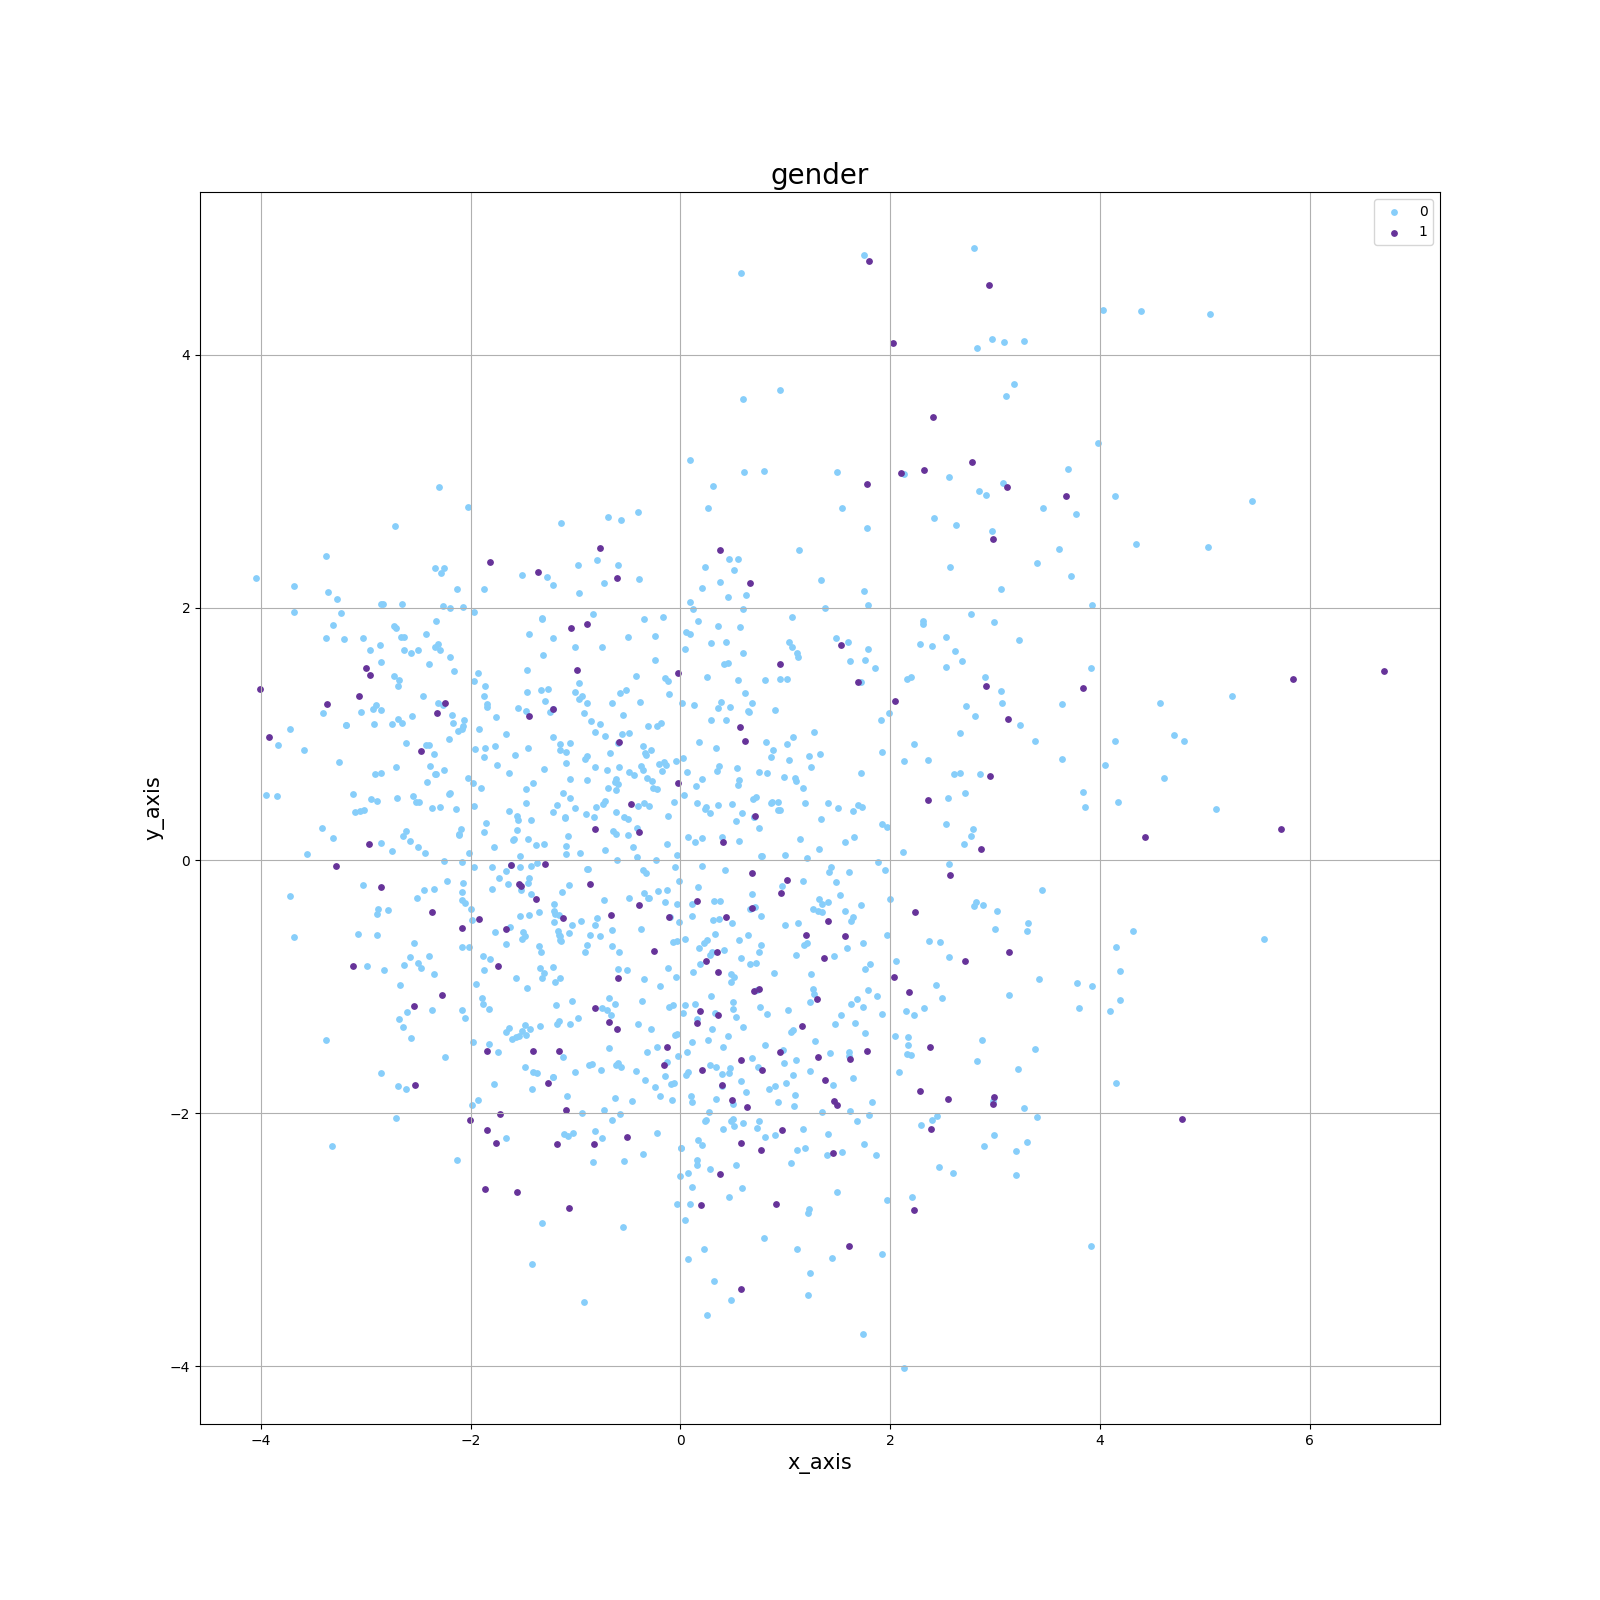
\includegraphics[width=\linewidth]{../img/administration_PCA_gender.png}
      \caption{PCA}
      \label{img::administration::gender::PCA}
    \end{subfigure}%
    \begin{subfigure}{.5\textwidth}
      \centering
      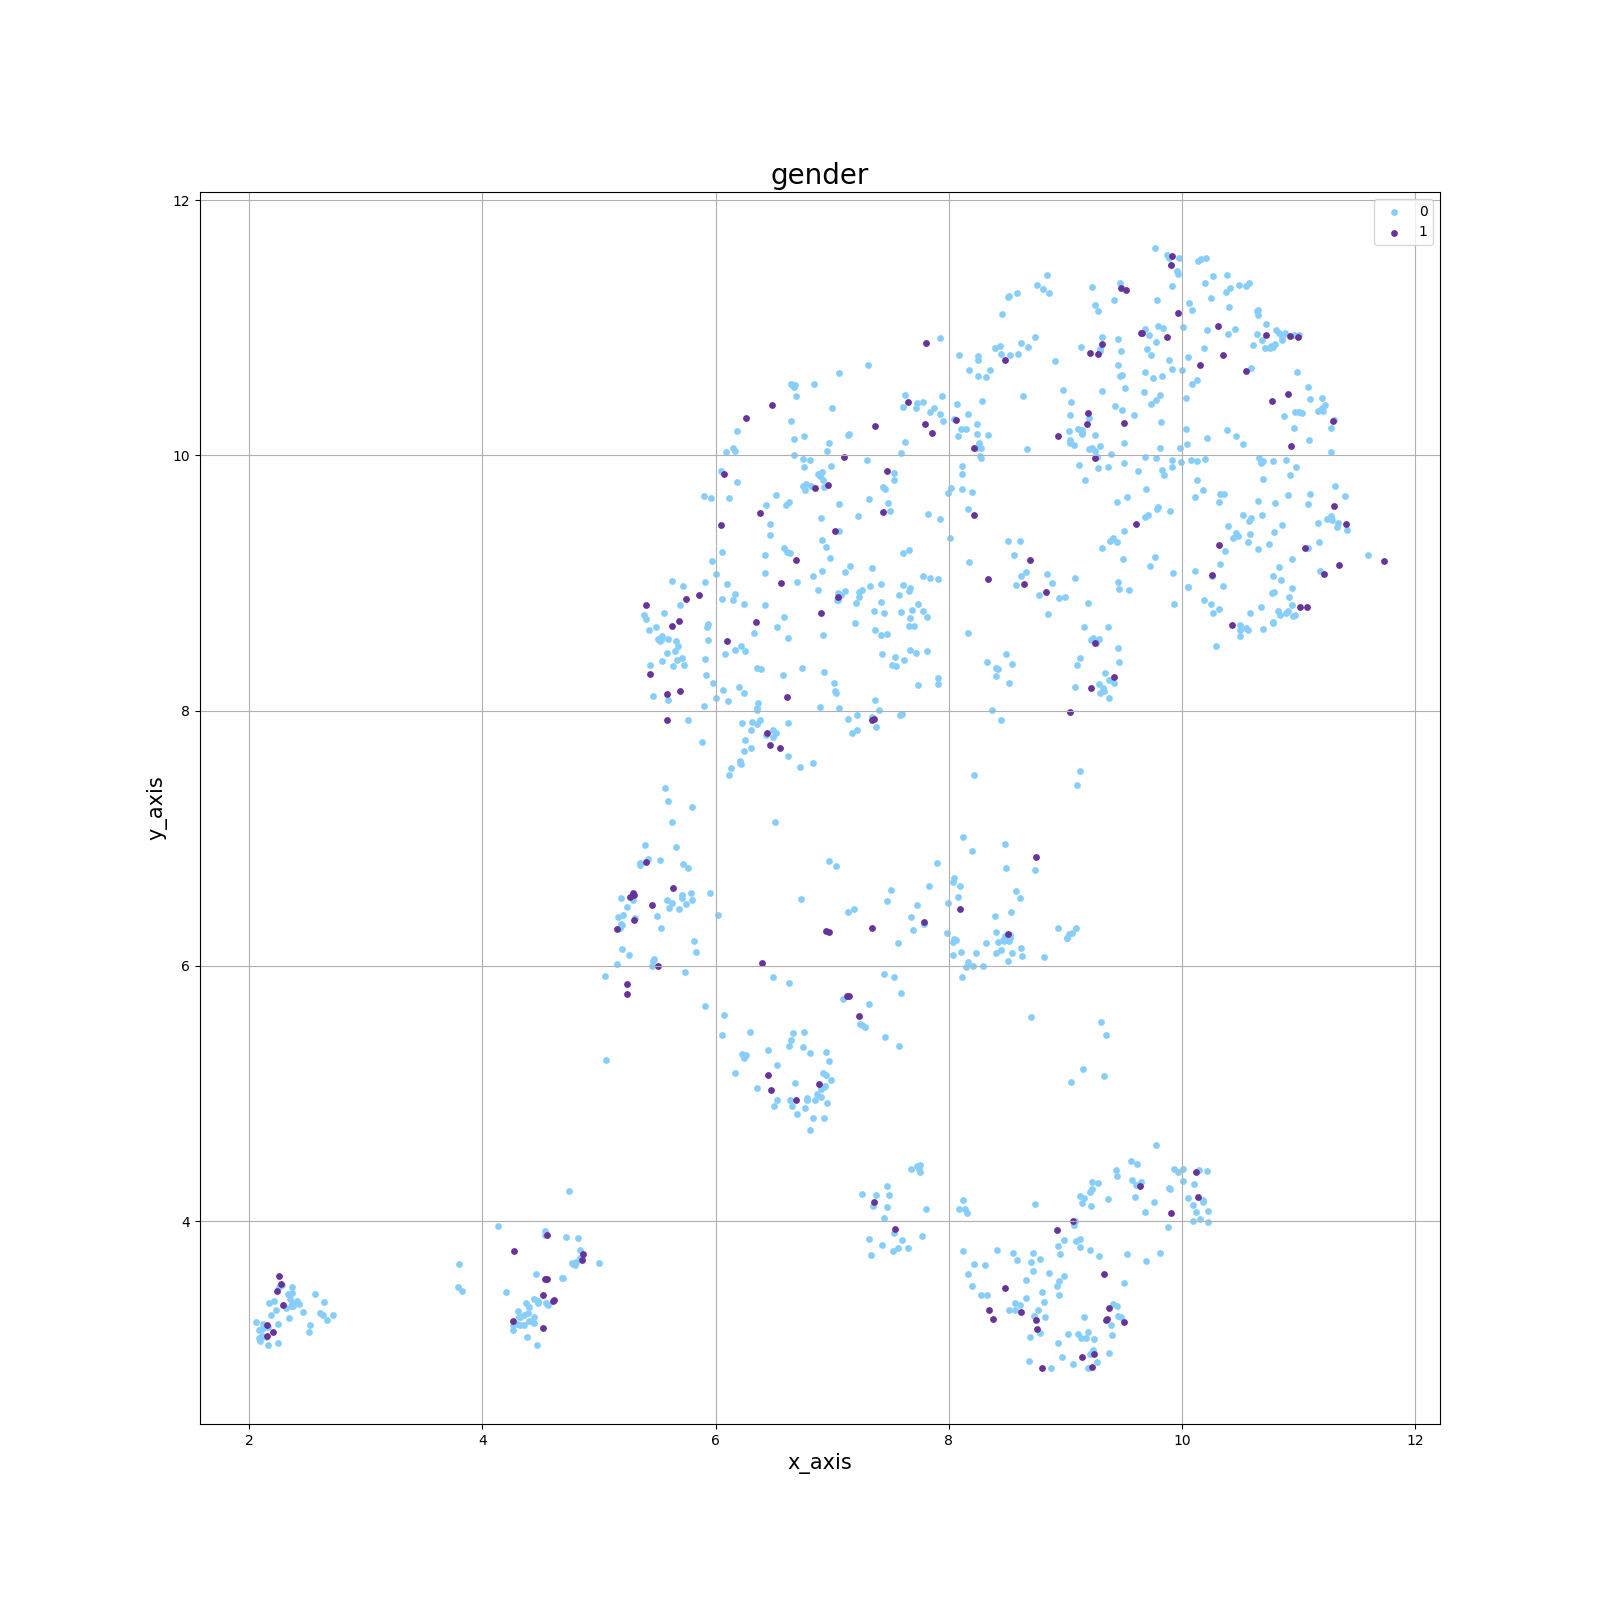
\includegraphics[width=\linewidth]{../img/administration_UMAP_gender.png}
      \caption{UMAP}
      \label{img::administration::gender::UMAP}
    \end{subfigure}
    \caption{Распределение ответов администрации в зависимости от пола}
\end{figure}

На построенных распределениях для администрации (рис. \ref{img::administration::gender::PCA} и \ref{img::administration::gender::UMAP}) мы можем видеть, что вне зависимости от гендера респондентов, распределяются по кластерам они примерно одинаково, с той лишь разницей, что женского персонала в составе администрации школ сильно больше, чем мужского.
Аналогичное распределение мы можем наблюдать и на ответах школьников (рис. \ref{img::students::gender::PCA} и \ref{img::students::gender::UMAP}), только в этом случае у нас примерно одинаковое количество респондентов разного пола.
Таким образом, гипотеза подтверждается, ответы участников действительно не зависят от пола.

\begin{figure}[h!]
    \centering
    
    \begin{subfigure}{.5\textwidth}
      \centering
      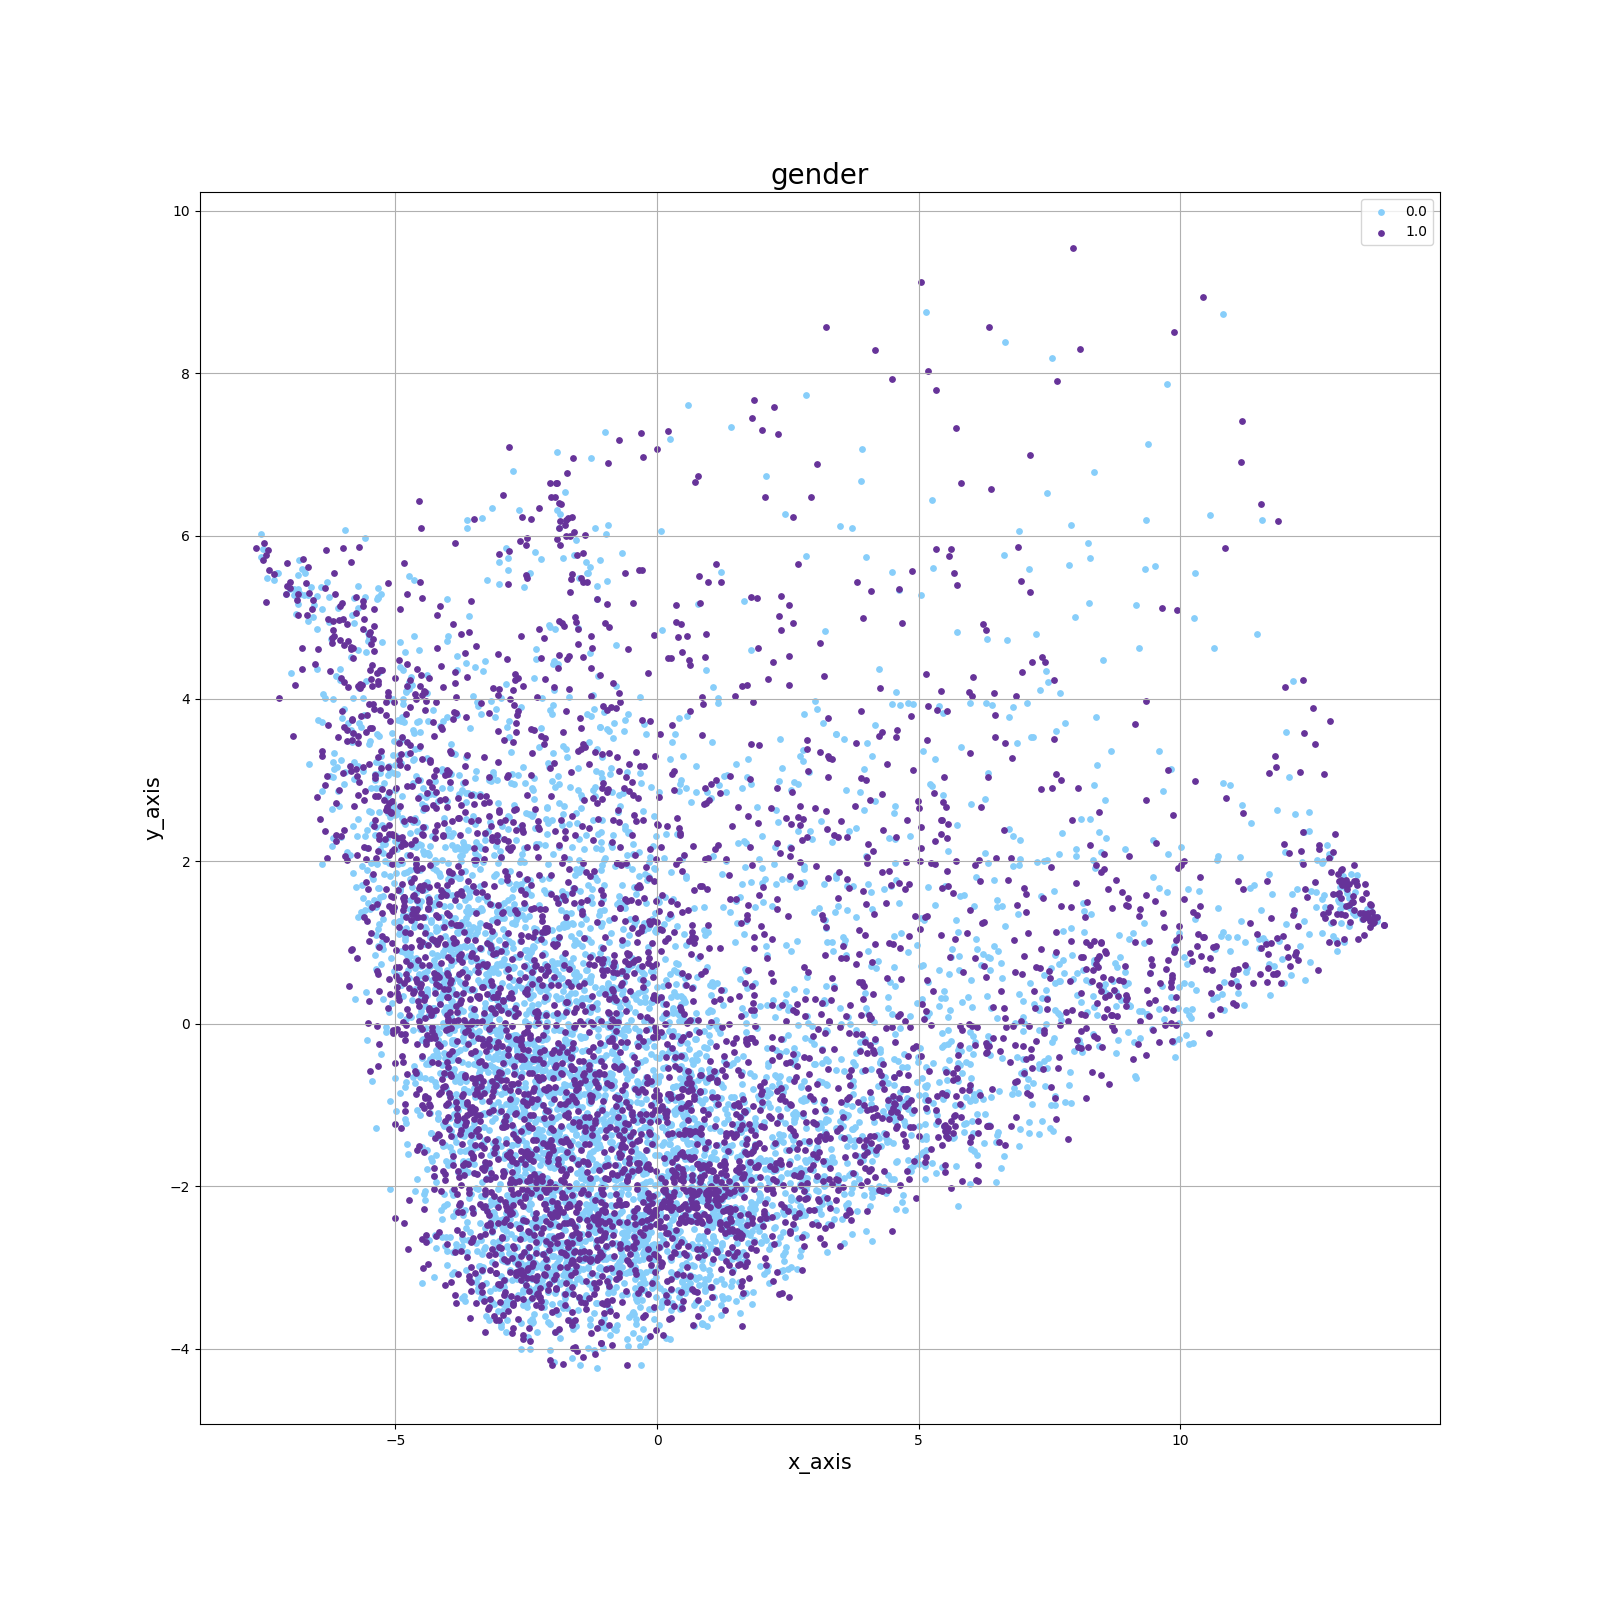
\includegraphics[width=\linewidth]{../img/students_PCA_gender.png}
      \caption{PCA}
      \label{img::students::gender::PCA}
    \end{subfigure}%
    \begin{subfigure}{.5\textwidth}
      \centering
      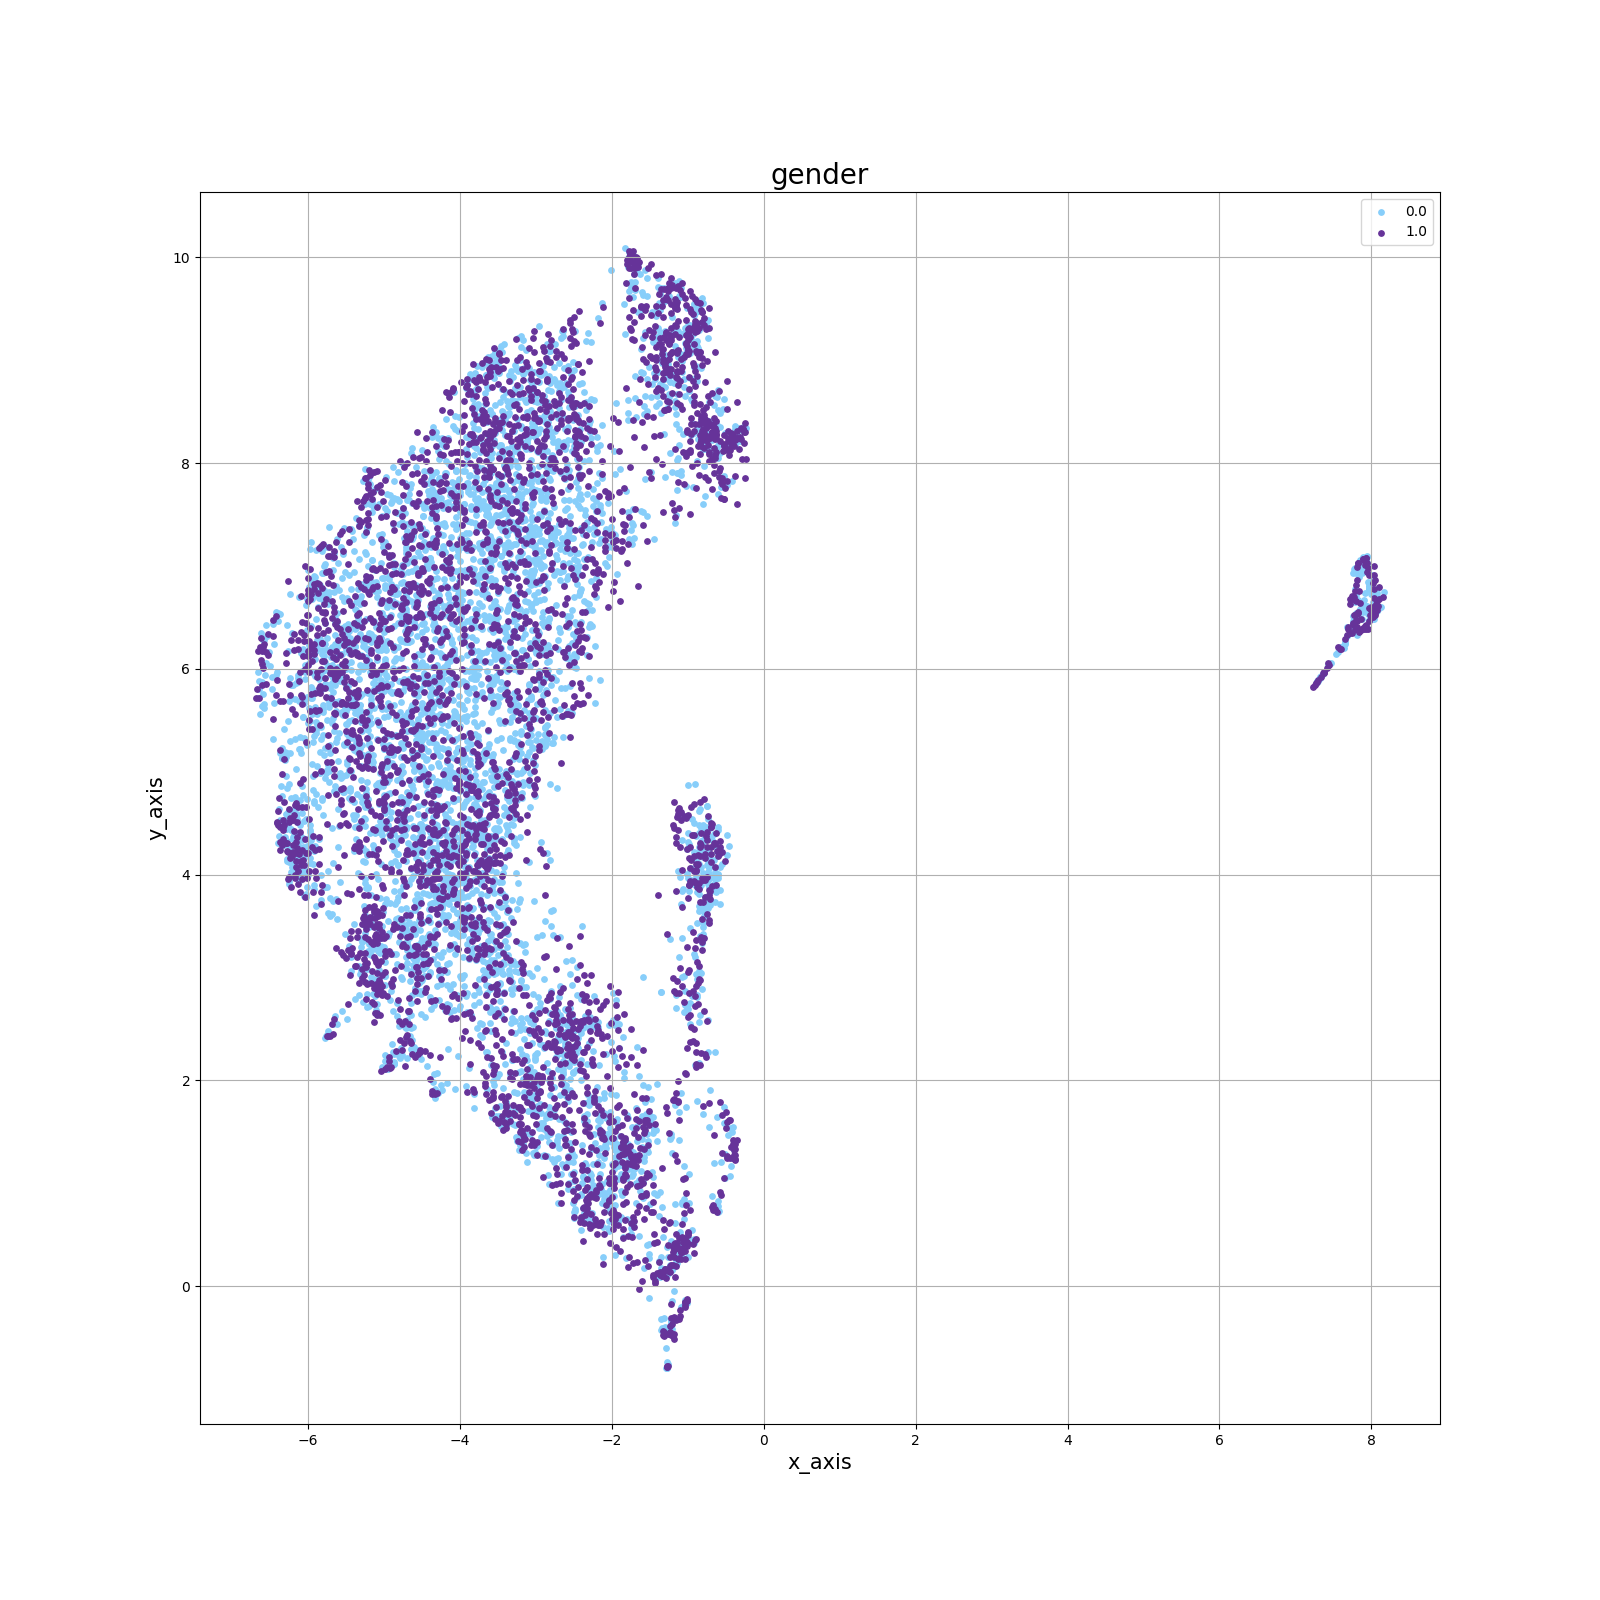
\includegraphics[width=\linewidth]{../img/students_UMAP_gender.png}
      \caption{UMAP}
      \label{img::students::gender::UMAP}
    \end{subfigure}
    \caption{Распределение ответов школьников в зависимости от пола}
\end{figure}

\subsection{Распределение ответов учеников на опрос не зависит от класса, в котором ученик обучается}

\begin{figure}[H]
    \centering
    \begin{subfigure}{.5\textwidth}
      \centering
      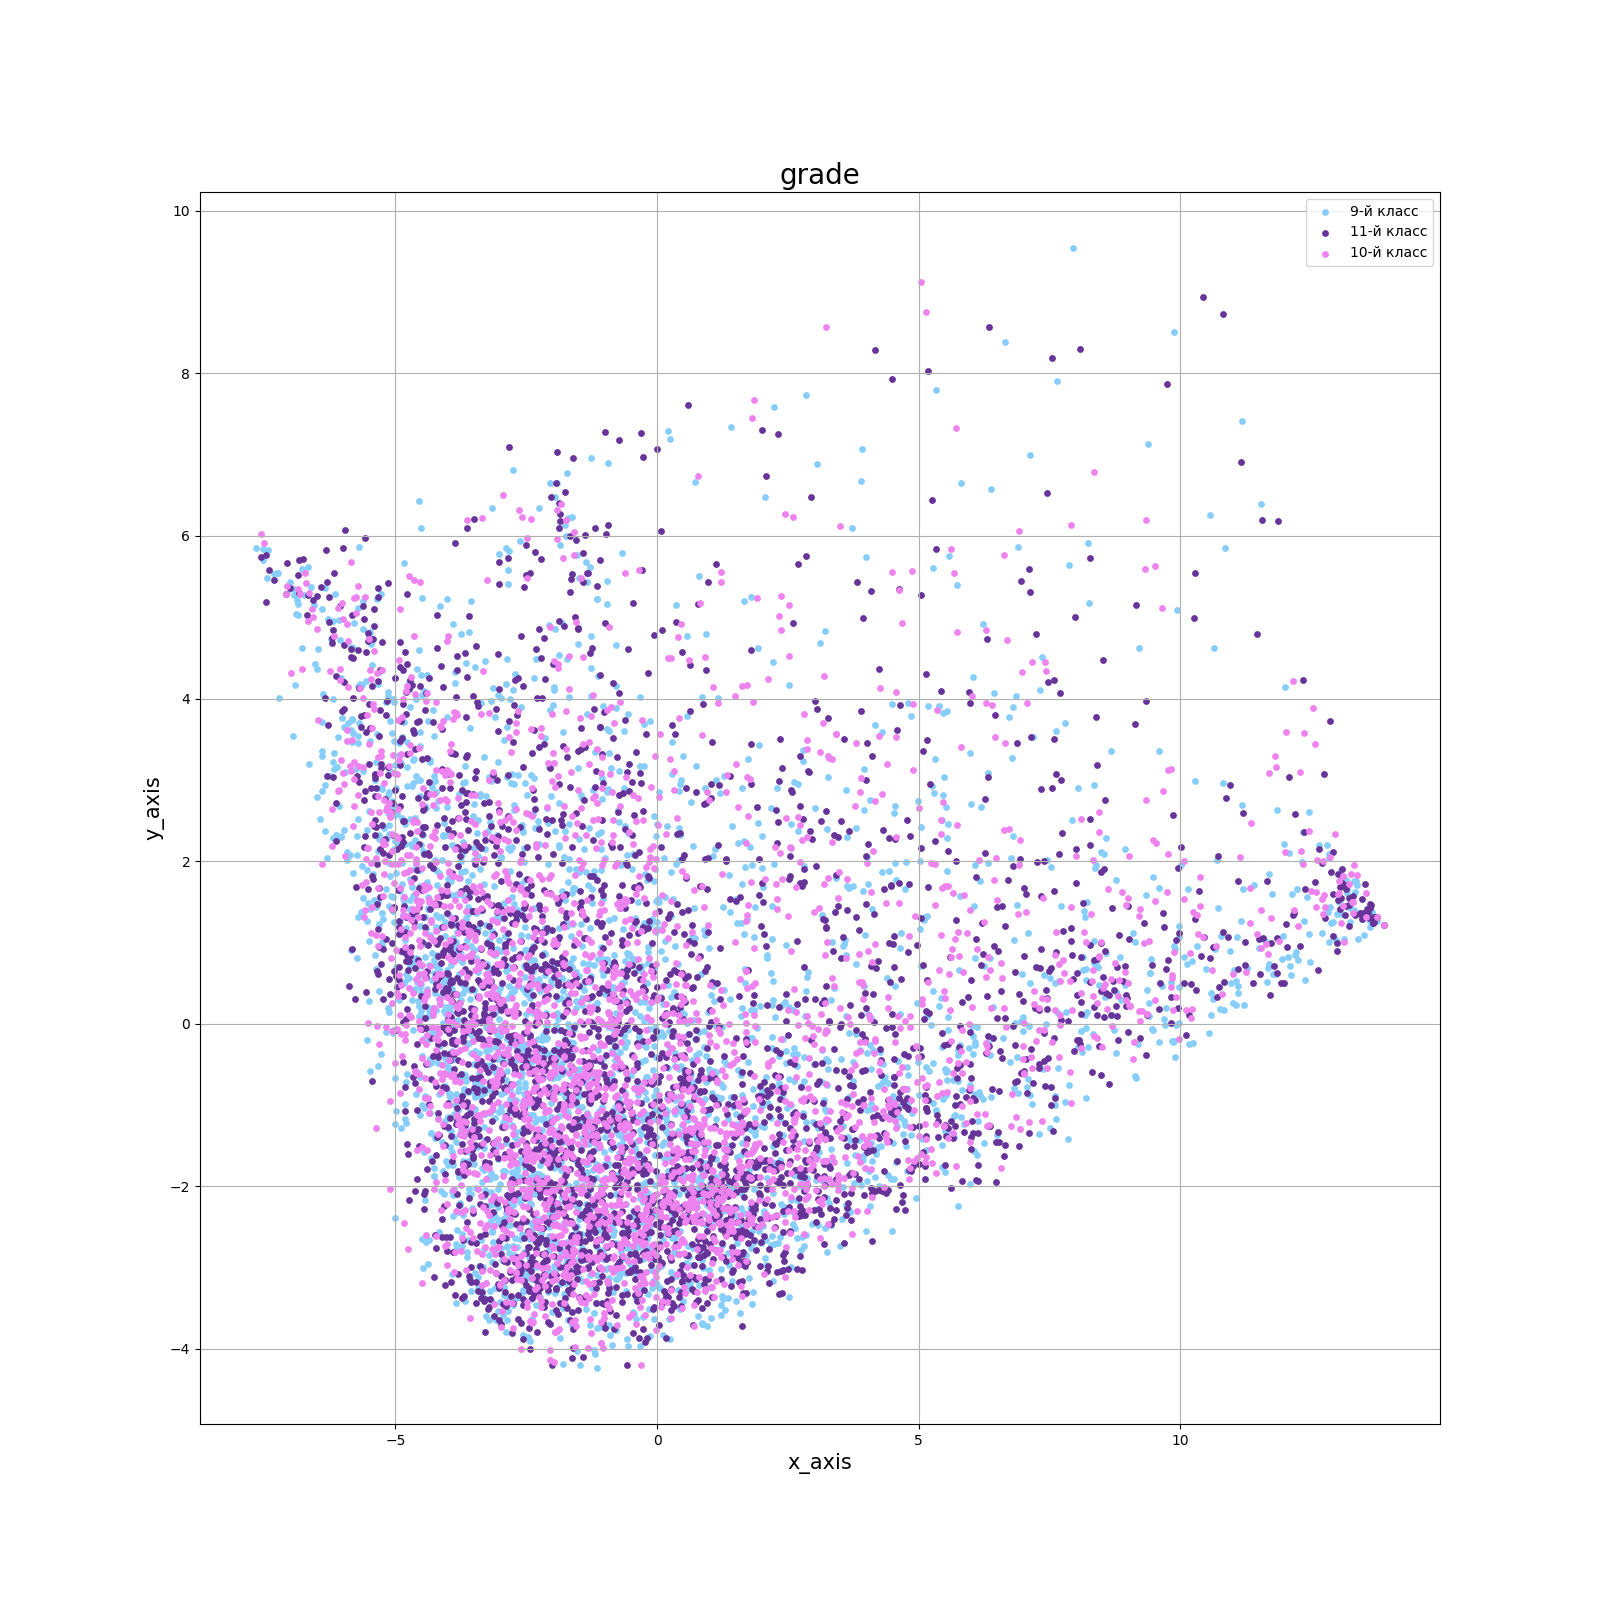
\includegraphics[width=\linewidth]{../img/students_PCA_grade.png}
      \caption{PCA}
      \label{img::students::grade::PCA}
    \end{subfigure}%
    \begin{subfigure}{.5\textwidth}
      \centering
      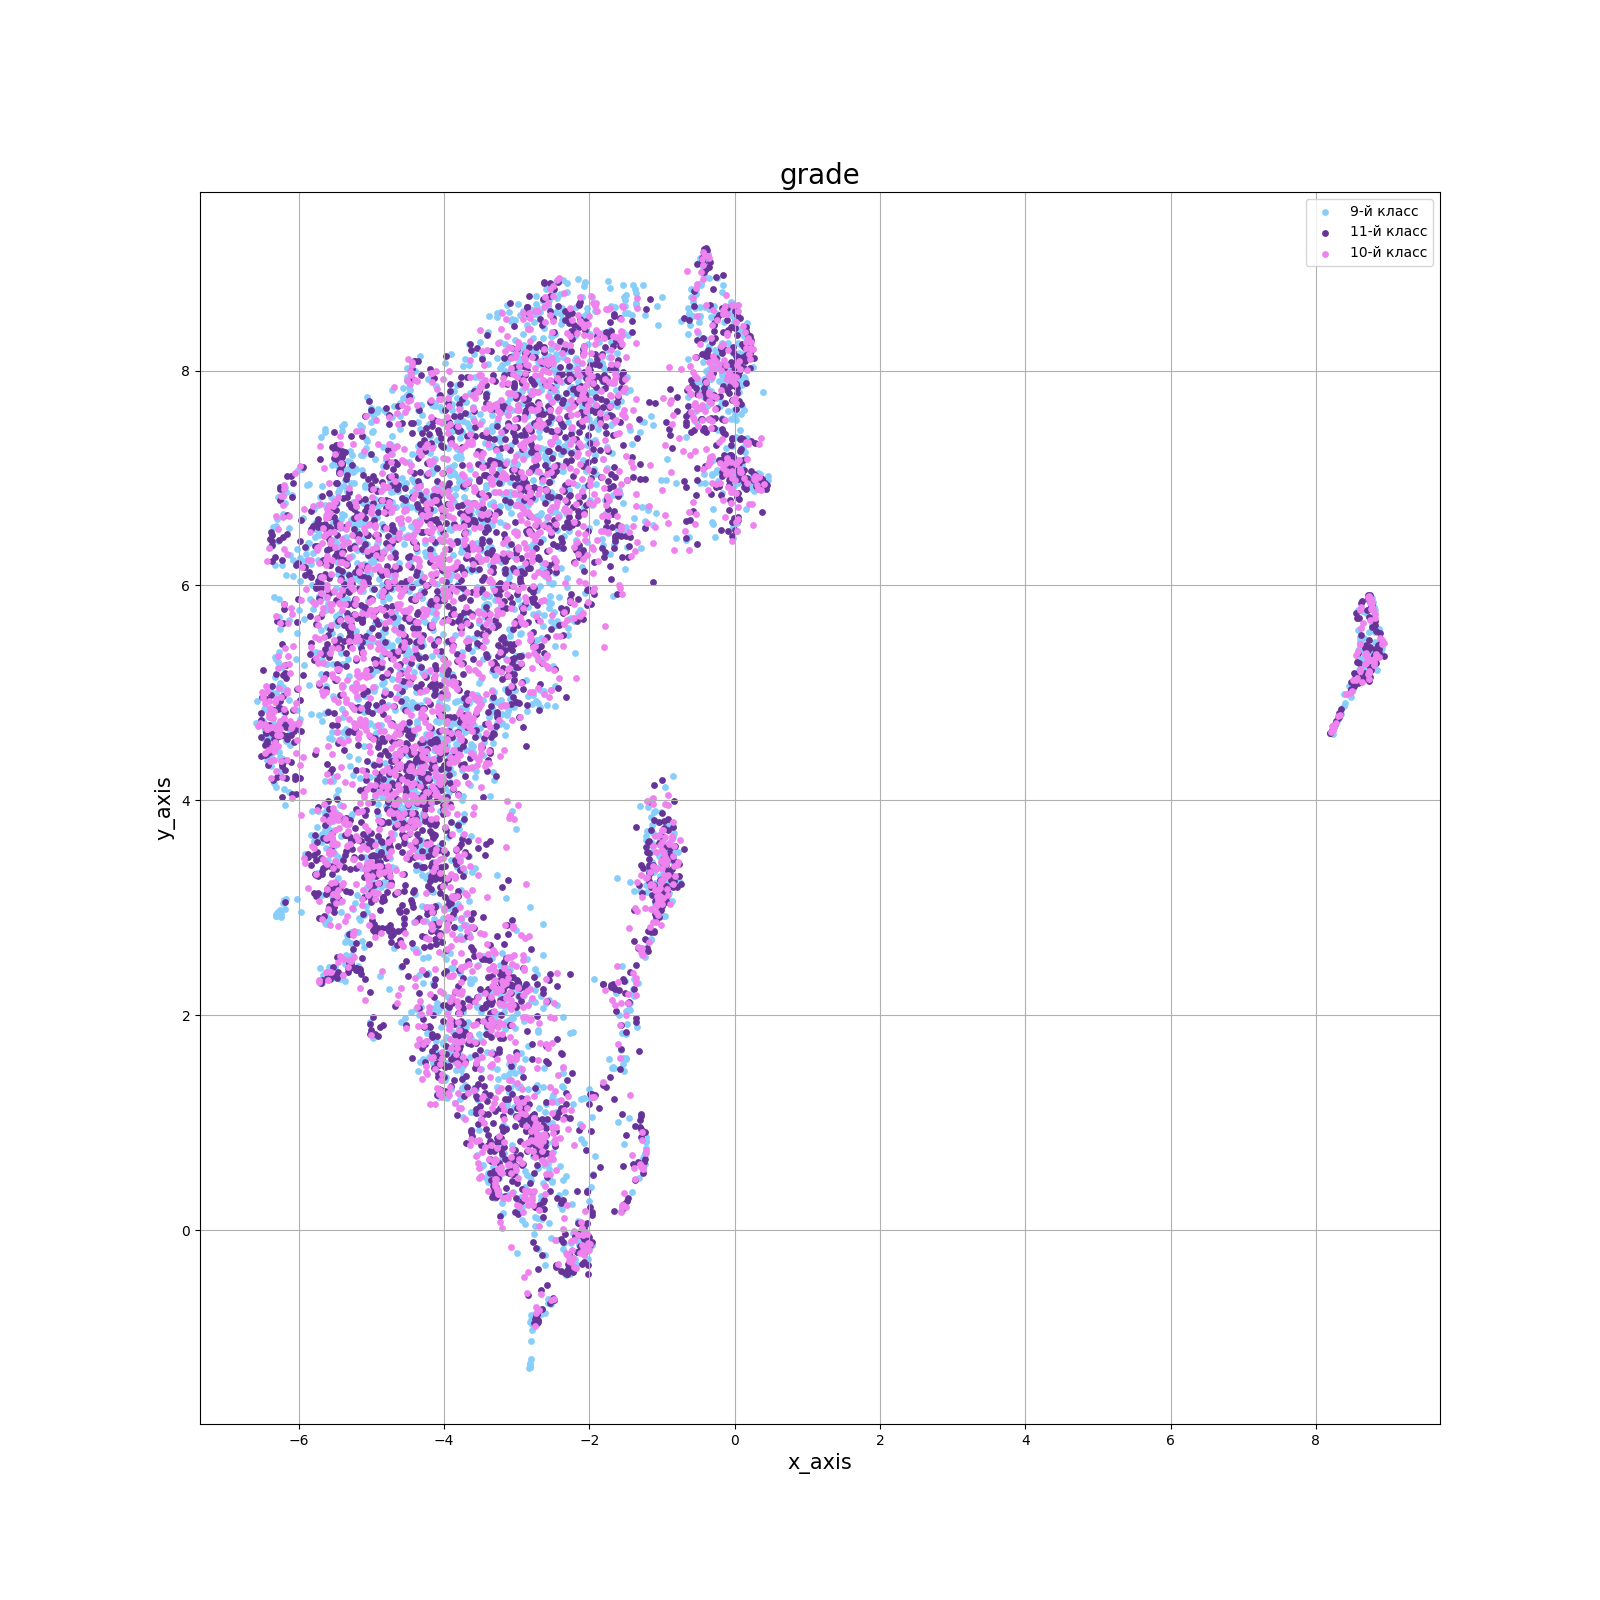
\includegraphics[width=\linewidth]{../img/students_UMAP_grade.png}
      \caption{UMAP}
      \label{img::students::grade::UMAP}
    \end{subfigure}
    \caption{Распределение ответов студентов в зависимости от класса}
\end{figure}

На рис. \ref{img::students::grade::PCA} и \ref{img::students::grade::UMAP} мы можем заметить две вещи:
\begin{enumerate}
    \item Распределение абсолютно не отличается от того, которое было в секции \ref{hypothesis::1}, что не удивительно, учитывая тот факт, что я просто подменил целевую переменную, по которой раскрашиваю точки в пространстве.
    \item Распределение по классам весьма равномерное в двух кластерах в случае рис. \ref{img::students::grade::UMAP}.
\end{enumerate}
Таким образом, класс учеников не влияет на их ответы в опросе про техническую оснащенность школы.
Это, на самом деле, весьма логично, ведь если школа использует IT технологии в образовательном процессе отдельной параллели, то она будет эти же технологии распространять и на все остальные параллели.

\subsection{Распределение ответов членов школьной администрации зависит от должности}

\begin{figure}[H]
    \centering
    
    \begin{subfigure}{.5\textwidth}
      \centering
      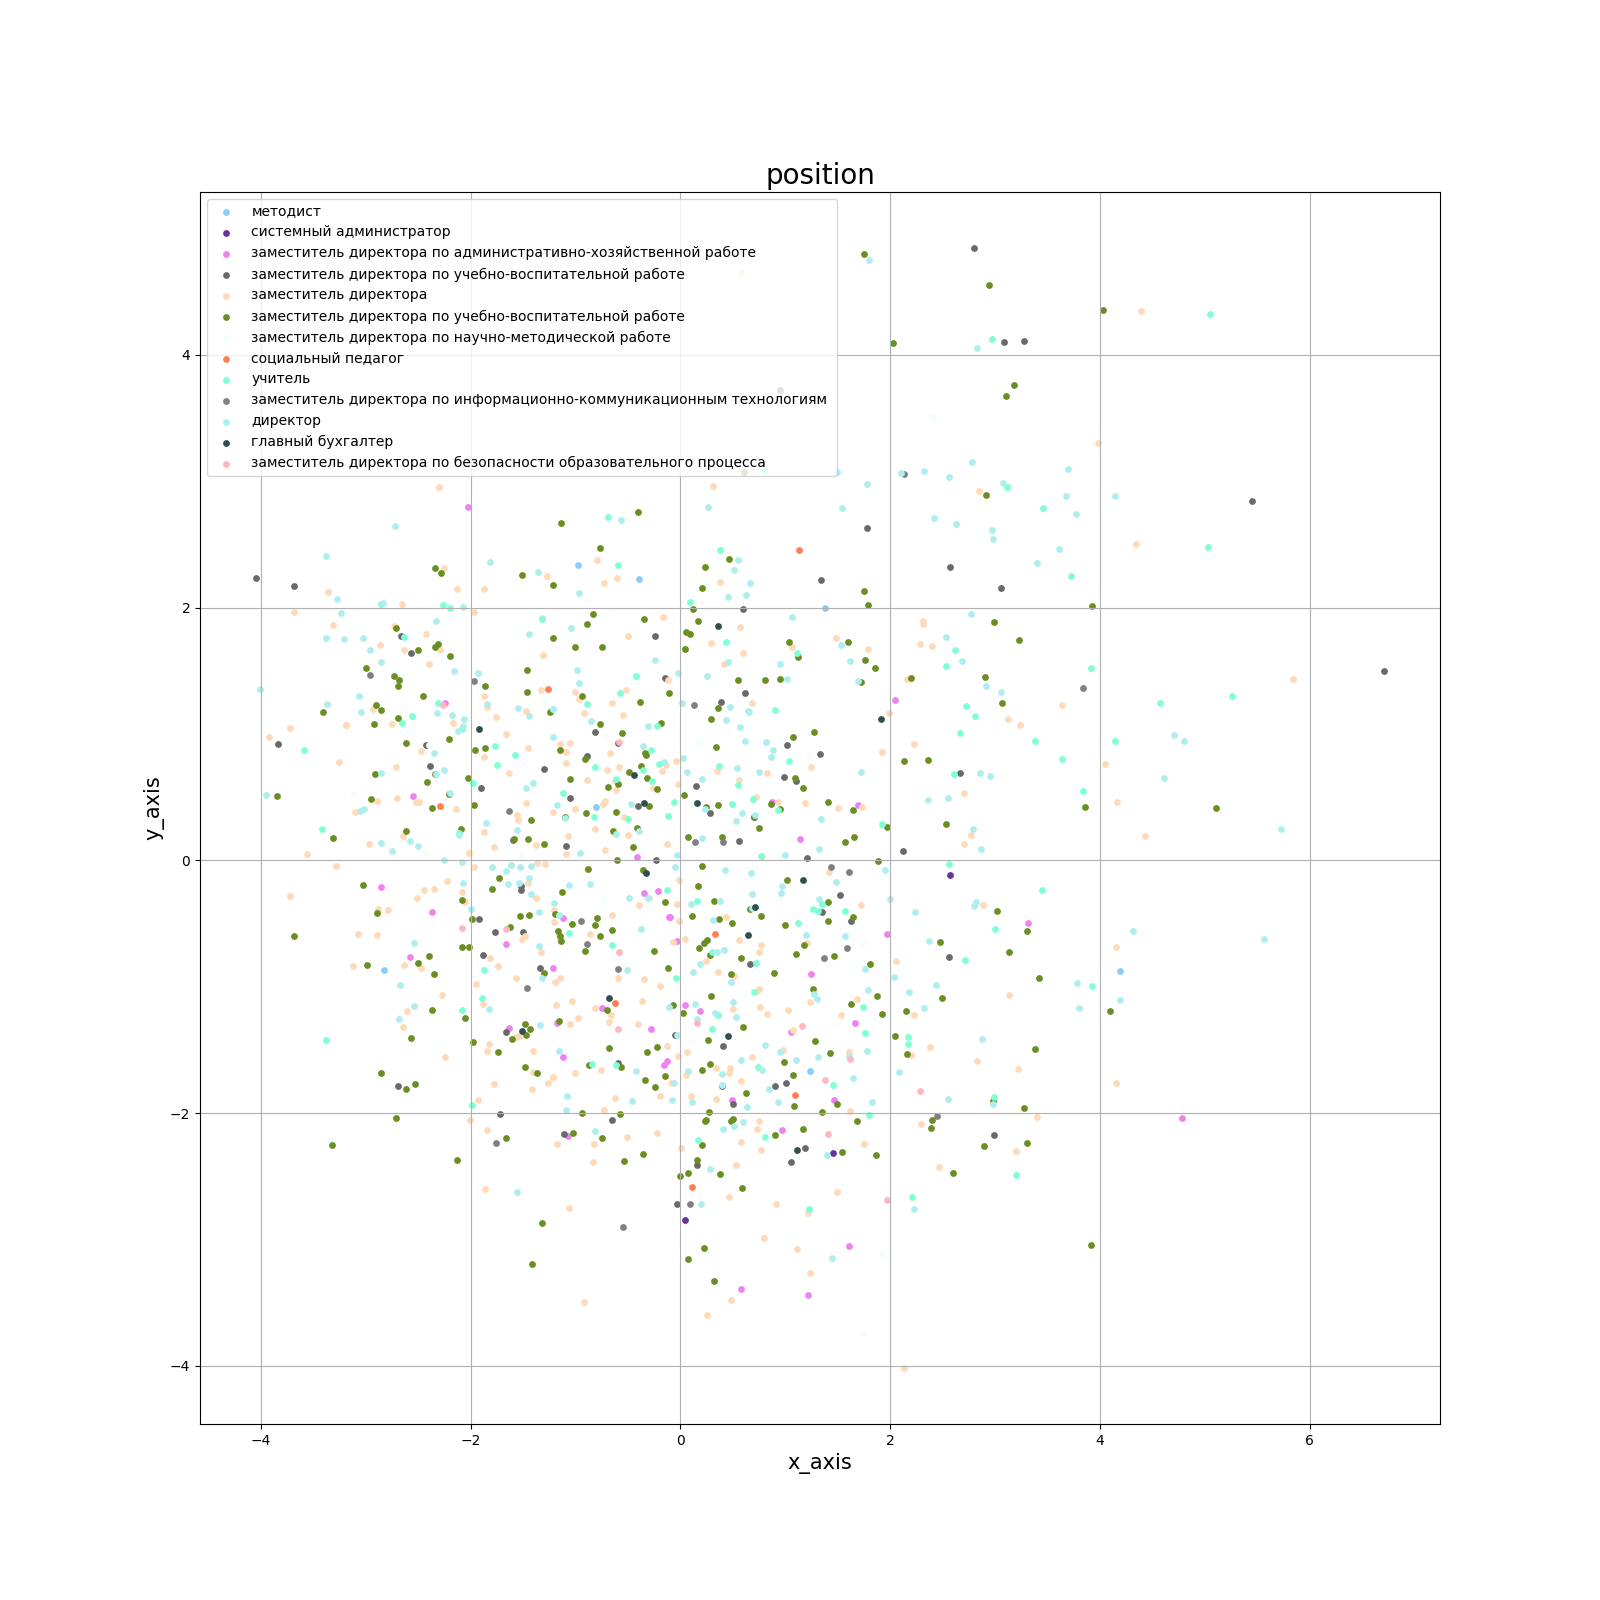
\includegraphics[width=\linewidth]{../img/administration_PCA_position.png}
      \caption{PCA}
      \label{img::administration::position::PCA}
    \end{subfigure}%
    \begin{subfigure}{.5\textwidth}
      \centering
      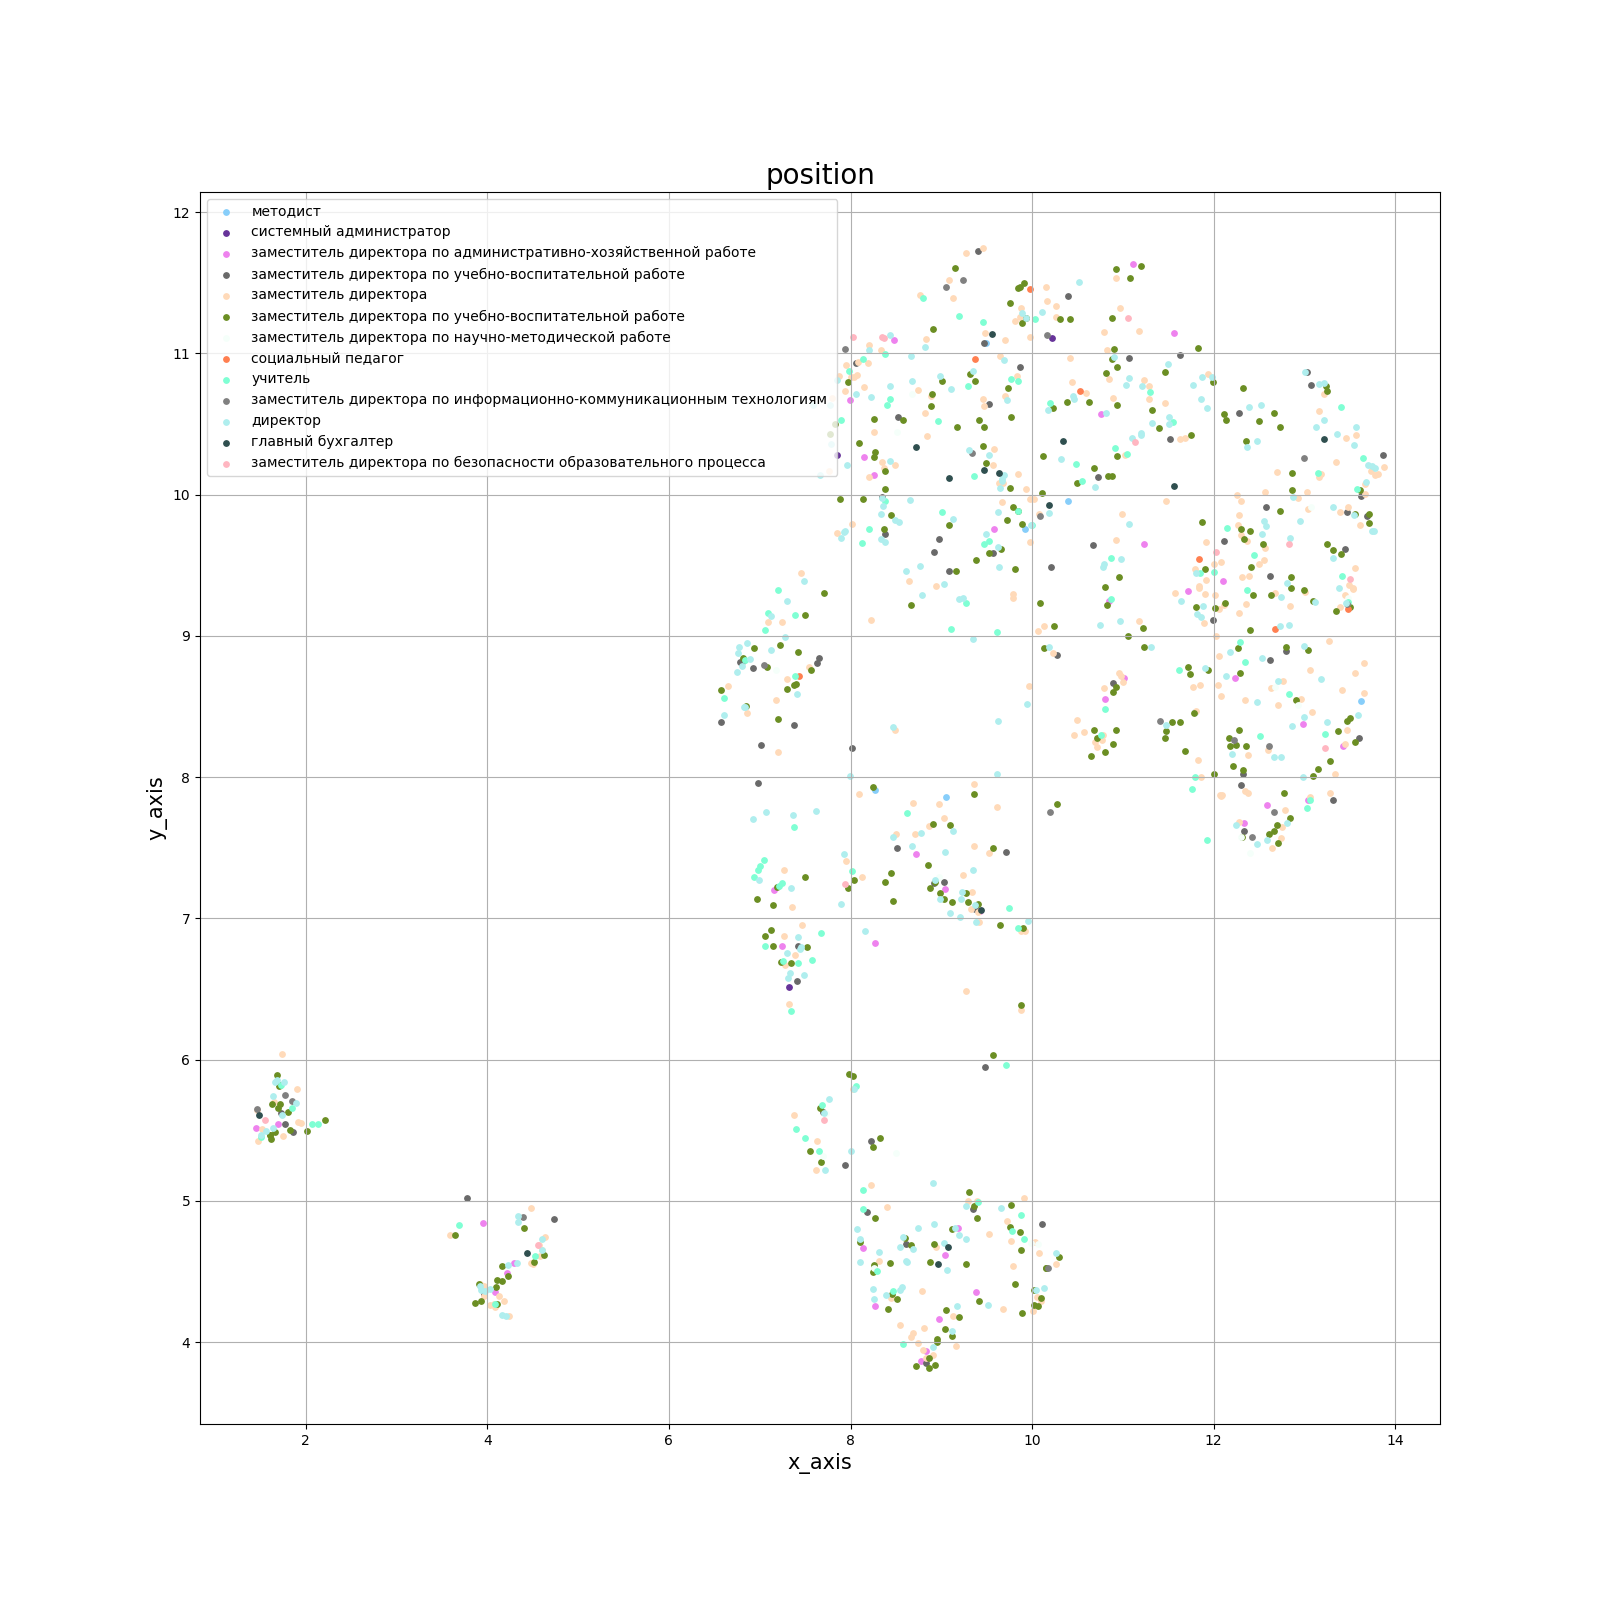
\includegraphics[width=\linewidth]{../img/administration_UMAP_position.png}
      \caption{UMAP}
      \label{img::administration::position::UMAP}
    \end{subfigure}
    \caption{Распределение ответов администрации школы в зависимости от должности}
\end{figure}

Как мы можем наблюдать, моя гипотеза не подтвердилась, поскольку почти все должности присутствуют в каждом из полученных кластеров на рис. \ref{img::administration::position::PCA} и \ref{img::administration::position::UMAP}.
Это говорит, как я предполагаю, о широкой осведомленности почти каждого сотрудника школьной администрации о технологической оснащенности школы.

\newpage
\section{План дальнейшей работы}

Следующей задачей является задача классификации респондентов в зависимости от их ответов.
Я попробую предсказывать школу человека по его ответам в опросе.
Также, в процессе предварительной обработки данных, я выбросил некоторые неструктурированные данные.
В частности, я проигнорировал все ответы на вопрос про использование конкретных электронных образовательных систем, хотя мне кажется, что в этих данных могут быть какие-то интересные закономерности.
Эти данные сложно поддаются обработке, однако я все равно попробую их почистить и по ним покластеризовать ответы участников опроса.

Также, планируется перебрать абсолютно все категориальные признаки, чтобы выявить, какой именно среди них влияет на образование кластеров среди ответов сотрудников школьной администрации (рис. \ref{img::administration::gender::UMAP}, \ref{img::administration::position::UMAP}).             % Вроде бы всё хорошо, это подходит под "Описание вычислительного эксперимента" почти идеально.
    % \section{Заключение}         % "Заключение. Основные результаты и выводы. Перспективы дальнейших исследований по теме."
    \printbibliography                                          % Надо объединить литературу из КТ1 и КТ2, добавить ещё некоторую
    \section{Приложение}

\begin{table}[h]
\centering
\caption{Календарный план работ по проекту}
\label{tab:project-plan}
\begin{tabular}{|p{0.35\linewidth}|p{0.6\linewidth}|}
\hline
Дата       & Название задачи                                                          \\ \hline
12.03.2021 & Ознакомление с методичкой по симплициальным комплексам и гомологиям      \\ \hline
22.03.2021 & Изучение работы классических алгоритмов анализа данных на соц. опросах   \\ \hline
30.03.2021 & Изучение работы топологических алгоритмов анализа данных на соц. опросах \\ \hline
14.04.2021 & Сравнительный анализ результатов и их визуализация                       \\ \hline
26.04.2021 & Отчет по КТ2                                                             \\ \hline
01.05.2021 & Изучение алгоритмов машинного обучения с учителем                        \\ \hline
07.05.2021 & Разработка модели (нейронной сети), которая будет предсказывать по ответам ученика его школу \\ \hline
15.05.2021 & Итоговый отчет по проекту                                                \\ \hline
\end{tabular}
\end{table}                              % По идеи, если работа будет финальной, то здесь вместо плана работы должны быть код, возможно

\end{document}
